%*******************************************************
% Step 1: Registration
%*******************************************************
\pdfbookmark[1]{Step 1: Registration}{Step 1: Registration}
\chapter{Step 1: Registration}

\setlength{\parindent}{0cm}

\section{Things to Know}
In order to use FollowThrough to its best potential you need to create an account on the web interface (detailed below). This will allow you to send all the data your computer records to the cloud so that you may review the recorded information later. All of the recorded data is contextualised and graphed for your viewing convenience.

\section{The Website}
The first step of the signing up process is to open up the web page. Start by opening up your browser of choice. Once it is open enter the url "http://54.145.183.186/" into the url bar (with no quotation marks) and press enter. You will be greeted by a page that looks like the one displayed below:
\begin{center}
    
\includegraphics[width = 1 \textwidth]{Pieces/home.PNG}
\end{center}

\section{Starting at Home}
When you arrive at the home page on the website you will notice a few things. Most obviously, the logo is displayed in the middle of the screen. However you will also notice the two buttons on the top left ([1] and [2] in the picture).

\begin{center}
    \includegraphics[width = 1 \textwidth]{Pieces/homeL.png}
\end{center}

\subsection{What These Buttons Do}

\begin{enumerate}[{[1]}]
\item is the log-in button. If you have already registered with an account this button is irrelevant to you. However if you have already registered skip to step 2.
\item is the register button. If you have not already registered for an account this button is the relevant one for you. Press this button to continue registering for an account.
\end{enumerate}

\section{The Registration Page}
After pressing the register button you will be met with a page that looks like this (except your page will not have labels):

\begin{center}
    \includegraphics[width = 1 \textwidth]{Pieces/registerL.png}
\end{center}

\subsection{Steps to Register}
Keep in mind that you may press the FollowThrough logo at the top left to return to the home page at any point of this process.

\begin{enumerate}[{[1]}]
\item The first step is entering your first and last name. These are case sensitive.
\item The second step is to enter your e-mail address. This has to be a unique e-mail which is not already in the system for security purposes.
\item The third step is to choose a password. It is recommended that you choose a password between 6-14 characters, containing at least one capitol letter, one lowercase letter, one number and one symbol. This will ensure that your password is strong.
\item Following that you must re-enter the exact password you used before. The two must match otherwise you will not be allowed to continue.
\item Finally, press the register button once all the other forms are complete to continue to the website.
\end{enumerate}

\\The website will automatically log you in after this process and send you to your home page which will look like this:

\begin{center}
    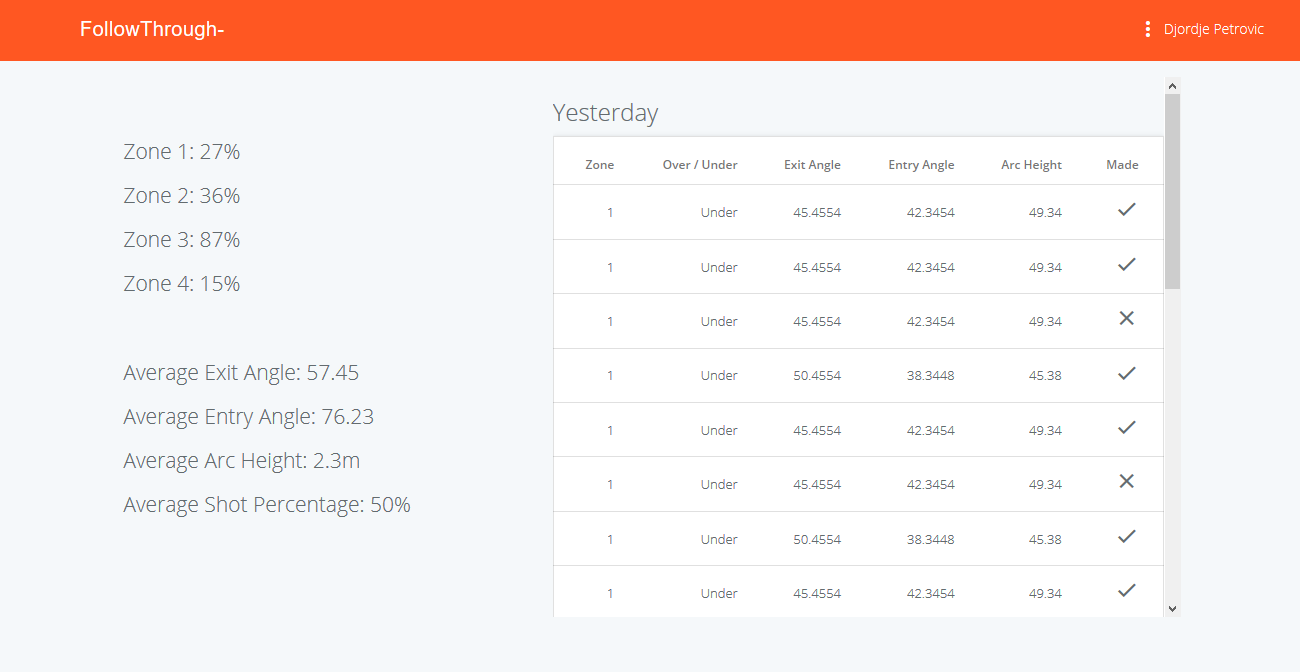
\includegraphics[width = 1 \textwidth]{Pieces/data.PNG}
\end{center}

\textbf{The contents of this page will be detailed at the end of step two.}